\documentclass[tikz, border=2pt]{standalone}

\usepackage{amsmath,amssymb}
\usepackage{pgfplots}
\pgfplotsset{compat=1.18}
\usepgfplotslibrary{groupplots}
\usetikzlibrary{arrows.meta}
\usepackage{xcolor}

\definecolor{utnblue}{RGB}{0, 51, 102}

\begin{document}
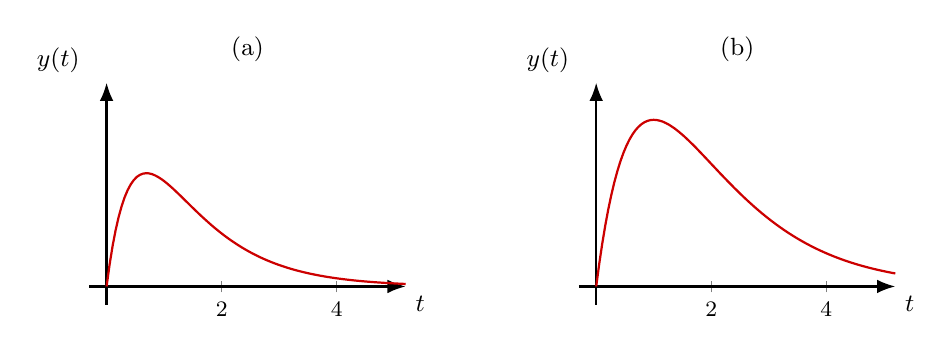
\begin{tikzpicture}[>=Latex, font=\small]

\pgfplotsset{
  every axis/.append style={
    axis lines=middle,
    axis line style={->, thick, black},
    width=5.6cm, height=4.4cm,
    xlabel={$t$}, ylabel={$y(t)$},
    xlabel style={anchor=north west},
    ylabel style={rotate=0, anchor=south east, at={(axis description cs:0,1)}},
    xmin=-0.3, xmax=5.2,
    ymin=-0.04, ymax=0.45,
    ytick=\empty,
    xticklabel style={font=\footnotesize},
    title style={yshift=-2pt},
    samples=100,
    clip=false,
  },
  resp/.style={red!80!black, thick},
  guia/.style={gray!55, thin, dashed},
}

\begin{groupplot}[
  group style={group size=2 by 1, horizontal sep=2.2cm},
]
  % ===== (a) a != b : diferencia de exponenciales =====
  \nextgroupplot[domain=0:5.2, title={(a)}]
    \addplot[resp] {exp(-x) - exp(-2*x)};

  % ===== (b) a = b : rampa amortiguada t e^{-at} =====
  \nextgroupplot[domain=0:5.2, title={(b)}]
    \addplot[resp] {x*exp(-x)};
\end{groupplot}
\end{tikzpicture}
\end{document}
